% \section{Fault Characterization} A detailed study of how the sensor works and its functional block diagram gives us an insight into detecting and characterizing the faults that could result from sensor failures.

% \subsection{Faults in PIR Sensors} A PIR sensor can fail in multiple ways. Broadly the failures could occur either in the lens subsystem, the pyroelectric subsystem or the component electronics in the sensor.  We closely analyze each of the subsystems in the sensor to flesh out the possible failures that can occur. It is be noted that we account for \textit{practical}, \textit{commonly observed} and \textit{most frequent} failures. Consequently, uncommon failures such as due to cosmic rays and alpha-particles are outside the scope of this discussion. Nevertheless, if the designer needs to account for esoteric failures, our framework provides a guideline for analysis. 

% \subsubsection{Failures in the lens subsystem} Typically, in commodity PIR sensors, the lens is geometrically constructed to precisely focus the infra-red rays into the pyroelectric element. As a result, any factor that affects the lens could result in loss of precision in focusing the infra-red rays can affect the accuracy of PIR sensors. Broadly we have seen three classes of failures in this space.

% \noindent \textbf{Lens cap dislocation:} Generally, the lens is either stuck onto the sensor board with an adhesive material (refer Fig. \ref{}) or is constructed with hooks that latch onto the the sensor board (refer Fig. \ref{}). Thus, as a result of this, in deployment, the lens could get dislodged from its place or completely fall off the sensor board due to factors such as thermal expansion or physical impact with a foreign object in the environment.

% \noindent \textbf{Lens cap deformation:} The lens is typically made of milky white, flexible, 0.4mm thick high density plastic \cite{fresnel}. Plastic material is susceptible to physical deformation due to factors such as physical impact that can change the shape or puncture the lens. The result is that this results in imperfect capture and focusing of the infra-red radiation that is incident on the surface of the sensor.

% \noindent \textbf{Lens cap hindrance:} Foreign material such as dust particles (\eg in case of factory floors) or objects such as paper and plastic can alter the behavior of the lens subsystem as the thermal absorption of the infra-red rays is now altered by the foreign object.   

% \subsubsection{Failures in the pyroelectric subsystem} The pyroelectric subsystem is another critical point of failure in a PIR sensor. The pyroelectric subsystem consists of an optical filter and a pyroelectric element (electrode) both of which are housed in an metallic enclosure with its output being wired to the remaining on-board electronics. The optical filter and pyroelectric element are prone to degradation with exposure to high temperature.

% \noindent \textbf{Optical filter damage:} The optical filter has an operational curve (transmittance as a function of wavelength) which is dependent on the temperature. The filter is designed to detect human motion and is carefully calibrated to trigger in the region of human motion. As a result, the filter is susceptible to damage due to environmental elements such as temperature and humidity which affect the operational characteristics.

% \noindent \textbf{Optical filter ageing:} TBD

% \subsubsection{Failures in the on-board electronics} The on-board electronics consisting of the amplifier and comparator circuitry are prone to all the failure modes of electronics \viz shorted pins, floating pins, and degradation due to elements such as temperature and humidity.




% The set of failures we consider are summarized in Table \ref{tab:pir_faults}. 

% \begin{table}[h]\footnotesize
% \renewcommand{\arraystretch}{1.1}
% \caption{Failures in a PIR Sensor}
% \label{tab:pir_faults}
% %\centering
% \begin{tabular}{p{2.50cm}||p{5cm}}
% \hline %\\
% \bfseries Failure & \bfseries Definition \& Impact\\
% \hline\hline
% \rowcol \bfseries Lens Subsystem & \\
% Lens cap dislodged \newline (Class I) & Lens cap could suffer partial dislocation or a complete drop off due to physical impact a foreign object or due to degradation of bonding \\
% Lens cap deformed \newline (Class II) & Lens cap could suffer physical damage in-place . \Eg deformation, puncture \etc \\
% Lens cap covered \newline (Class III) & Lens cap could be physically obstructed due to foreign particles from the environment. \Eg paper, tape or dust \\
% \hline
% \rowcol \bfseries Pyroelectric Subsystem & \\
% Pyroelectric Window damage (Class IV) & Pyroelectric Window could get damaged due to enviromental factors such as temperature or humidity\\
% Pyroelectric Element Ageing (Class VI) & Pyroelectric element can degrade or age and can give imperfect output\\
% \hline
% \rowcol \bfseries On-board Electronics & \\
% Electronic faults \newline (Class V) & The electronics could suffer from faults, \eg short circuits, floating outputs, \\
% % Thermal Faults & Pyroelectric element can degrade or age and can give imperfect output\\
% \hline
% \end{tabular}
% \end{table}




% \begin{table}[h]\footnotesize
% \renewcommand{\arraystretch}{1.1}
% \caption{Movement Patterns in the Deployment Scenarios used for evaluation}
% \label{tab:movement_patterns}
% %\centering
% \begin{tabular}{p{3.50cm}||p{4cm}}
% \hline %\\
% \bfseries Deployment Scenario & \bfseries Movement Patterns\\
% \hline\hline
% \rowcol \bfseries Elevator at CSL, Illinois & \\
% Deployment duration : 5 days \newline At: Inside Elevator of 4 floors on the Sidewalls & Motion category: smooth motion, mostly 2-3 people at a time, duration of occupancy approximately 20-30 seconds\\
% \hline
% \rowcol \bfseries Lobby at CSL, Illinois  & \\
% Deployment duration : 5 days \newline At: On sidewalls of lobby with chair and tables & Motion category: smooth motion, mostly one person at a time, can have people sit sometimes \\
% \hline
% \rowcol \bfseries Cafeteria during Lunch hour, Bangalore & \\
% Deployment duration : 1 hour \newline At: Near the food counter & Motion category: ragged motion, groups present \\
% \hline
% \rowcol \bfseries Queue of a coffee shop,  & \\
% Deployment duration : 4 hours \newline At: Entrance to the ordering Queue & Motion Category: linear motion entry/exit, no crowding \\
% \hline
% \end{tabular}
% \end{table}



%%%%%%%%%%%%%%%%%%%%%%%%%%%%%
% REPLACING TABLE WITH A FIGURE
%%%%%%%%%%%%%%%%%%%%%%%%%%%%%

% \begin{table}
% \small
% \parbox{.95\linewidth}{
% \centering
% \begin{tabular}{m{1cm} m{1cm} m{1cm} m{1cm} m{1cm} m{1cm}}
% \hline
%             & Lens Cap Dislodged & Lens Cap Covered & Pyroelectric Element Broken &  Pyroelectric Element Covered & Working \\\hline \hline
%     Lens Cap Dislodged & 1.0 & 0.0 & 0.0 & 0.0 & 0.0031 \\
%     Lens Cap Covered & 0.0 & 1.0 & 0.0 & 0.0 & 0.0  \\ 
%     Working Sensor & 0.0031 & 0.0 & 0.99 & 0.0031 & 0.0  \\
%     Pyroelectric Element Broken & 0.0 & 0.0 & 0.0 & 1.0 & 0.0 \\ 
%     Pyroelectric Element Covered & 0.0 & 0.0 & 0.0 & 0.0 & 1.0 \\ \hline 

% \hline
% \end{tabular}
% \caption{Elevator Deployment Classification of Faults Using Random Forest Classifier.}
% \label{tbl:elevator_classification_results}
% }
% \end{table}


% \subsection{Analysis of Deployment Results} We classify the results into 4 categories based on the time of deployment -- \ca No obstacle, deployed during the day, \cb With obstacle.

% %\begin{wrapfigure}{R}{0.65\textwidth}
% \begin{figure}%{R}{8cm}
% 	%\vspace*{-\baselineskip}
% 	%\begin{flushleft}
% 	%    	\begin{minipage}[t]{0.65\textwidth}
% 	%\centering
% 	\includegraphics[scale=0.5]{figures/2-PIR-Fault/all-5-combined/untitled-thick.png}
% 	%\vspace*{-1.0\baselineskip}
% 	\caption{\textbf{CDF of FFT Coefficients} showing different distributions depending on the class of faults.}
% 	%\vspace*{-0.25\baselineskip}
% 	\label{fig:cdf_combined_all}
% 	%    	\end{minipage}
% 	%\end{flushleft}
% 	%\vspace{-\baselineskip}
% \end{figure}
% %\end{wrapfigure}


\begin{figure*}%[t]
	%\centering
% 	\vspace{-1\baselineskip}
	\begin{subfigure}[t]{0.41\textwidth}
		%\centering
		%\includegraphics[width=\linewidth]{figures/2-PIR-Fault/all-5-combined/CDF_FFT_small.png}
		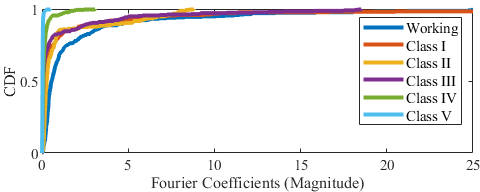
\includegraphics[width=\linewidth]{figures/2-PIR-Fault/all-5-combined/CDF_FFT.png}
		\caption{}
		\label{fig:cdf_combined_all}
	\end{subfigure}\hfill%
	\begin{subfigure}[b]{0.16\textwidth}
		\centering
		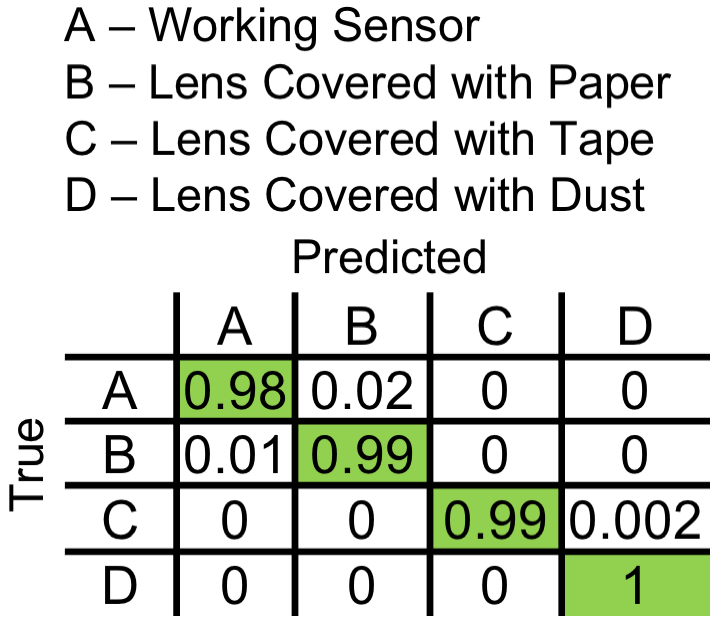
\includegraphics[width=\linewidth]{figures/classification/LensDefects/confusion-matrix-lensdefects.png}
		\caption{}
		\label{fig:finegrained_classification_results}
	\end{subfigure}%			
	\begin{subfigure}[t]{0.41\textwidth}
		\centering
		%\includegraphics[width=\linewidth]{figures/classification/LensDefects/Aout_Paper_Plastic_Dust_Normal.png}
		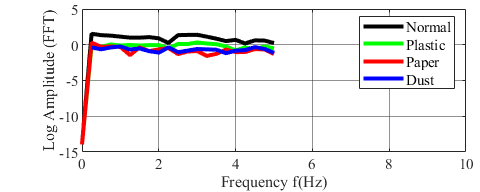
\includegraphics[width=\linewidth]{figures/classification/LensDefects/Log_Aout_Paper_Plastic_Dust_Normal.png}
		\caption{}
		\label{fig:finegrained_aout}
	\end{subfigure}
	\caption{\footnotesize{(a) CDF of FFT Coefficients showing different distributions depending on the class of faults.,(b) Fine-grained Fault Analysis,(c) \textbf{\aout} waveforms showing different behavior for paper, plastic and dust obstructions.}
	}
	\label{}
\end{figure*}

\subsection{Stage II -- Failure Diagnosis} 

Diagnosing the \textit{cause of failures (\ie class)} requires further investigation of \aout from faulty sensors.
%to reason about the \textit{class of the failure} according to our taxonomy. 
%
We combine our understanding of the PIR sensor \ie physics from \S\ref{subsec:physics}, failure taxonomy from \S\ref{subsec:taxonomy} and the frequency analysis of failures from \S\ref{subsec:freq_char} and feature analysis from \S\ref{subsec:bh} -- \S\ref{subsec:shap}. 
%
{\bfseries Fig.~\ref{fig:cdf_combined_all}} plots the CDF of FFT coefficients obtained for working sensors and various faulty sensors. 
%
The figure shows that although the distribution of working sensors (bottom-most curve) is distinct from failed sensors, different classes of failures have distributions that are not easily separable. 
%
Thus, relying on merely the FFT is insufficient. 
%
Consequently, we look at an additional 10 features as described in \S\ref{subsec:bh} --- \S\ref{subsec:shap} and shown in {\bfseries Fig.~\ref{fig:BH_feature_selection}}. 
%
%Failure diagnosis leverages the combined feature space to identify failure classes according to the taxonomy in \S\ref{subsec:taxonomy}.
%
%the subsystem that contains the failure and the type of failure (\eg lens fallen off, lens covered~\etc).
%We saw in each of the deployments that the we were able to identity the type of failure correctly.  
%

% \begin{figure}%{R}{7cm}
% 	%\vspace{-10pt}
% 	\begin{minipage}[t]{0.48\textwidth}
%     	\centering
%     	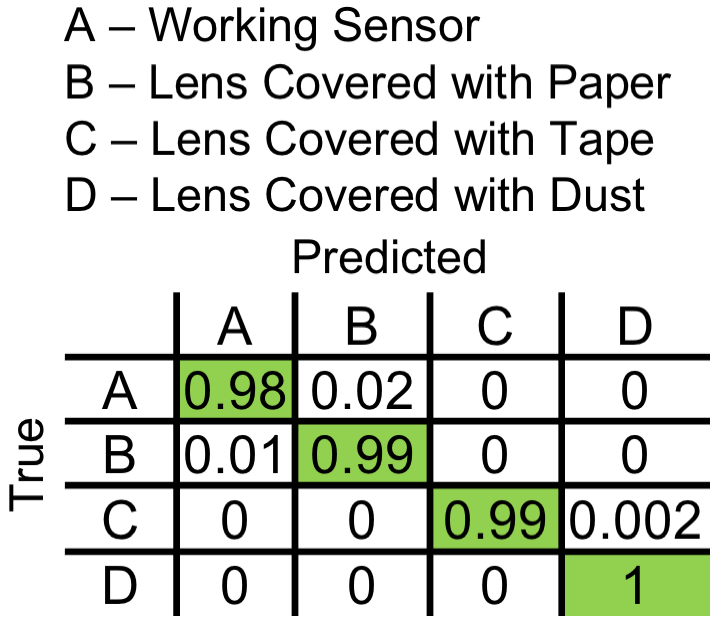
\includegraphics[width=\textwidth]{figures/classification/LensDefects/confusion-matrix-lensdefects.png}
% 	\caption{\textbf{Fine-grained} Fault Analysis}
% 	\label{fig:finegrained_classification_results}
% 	\end{minipage}%
% 	\hspace{1ex}
% 	\begin{minipage}[t]{0.48\textwidth}
% 		\centering		
% 		\includegraphics[width=\textwidth]{figures/classification/LensDefects/aoutwaveforms.png}
% 		\caption{\textbf{\aout} waveforms showing different behavior for paper, plastic and dust obstructions.}% allowing them to be separated.}
% 		\label{fig:finegrained_aout}
% 	\end{minipage}
% 	%\vspace{-10pt}
% \end{figure}

%This is also in line with the observations in \S\ref{subsec:learnability}. 
We validated this across the multiple deployments in the wild --- Elevator (\S\ref{subsubsec:elevator}), Lobby (\S\ref{subsubsec:lobby}), Starbucks (\S\ref{subsubsec:starbucks}) and Cafeteria (\S\ref{subsubsec:cafeteria}).
%, where we show detection and diagnosis of faults. 
%
%Thus, we are able to reason between different classes of faulty sensors by analyzing the features in addition to the FFT of the \aout waveform.
%
%\textbf{Note:}
Our real-world measurements demonstrate that features of \aout extracted during training and B-H feature selection is robust to variations in shapes and sizes of obstacles.

\begin{comment}
\begin{tcolorbox}[left=1pt,right=1pt,top=1ex,bottom=1pt,boxsep=0pt,
toptitle=0.5ex,bottomtitle=0.5ex]
{\bfseries Summary:} \ins{ML-based models developed considering multiple direct and derived time and frequency domain signal characteristics of \aout are required to diagnose the root cause of the failure in the sensor and point to the subsystem containing the failure.}
\end{tcolorbox}
\end{comment}

%The goal of this section is to identify faults from \S\ref{subsec:taxonomy} and point to the class of fault present in a particular sensor using the frequency domains analysis from \S\ref{subsec:freq_char}
%\vspace{-12pt}%was -15 pt
\subsection{Stage III -- Fine-Grained Failure Analysis} In fine-grained fault analysis, we point to the \textit{precise reason} for the fault where applicable. For example, in Class III faults it is useful to distinguish between different foreign substances contaminating the lens that can cause poor performance.
%the obstacles to be completely missed and lead to poor performance.

% \begin{wrapfigure}{R}{7cm}
% 	\vspace{-10pt}
% 	\centering
% 	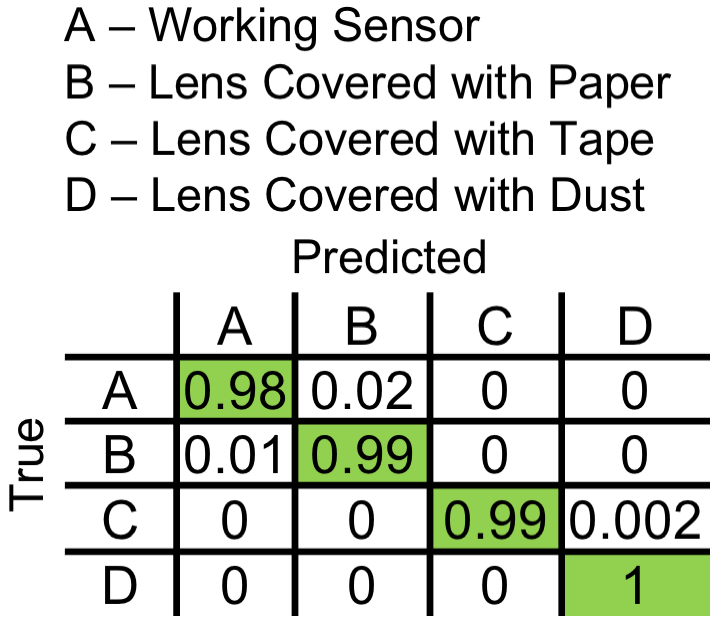
\includegraphics[width=7cm]{figures/classification/LensDefects/confusion-matrix-lensdefects.png}
% 	\caption{\textbf{Fine-grained} Fault Analysis}
% 	\label{fig:finegrained_classification_results}
% \end{wrapfigure}

To investigate this, we selected the set of faulty sensors identified as Class III faults in 
%the deployments in elevator, lobby and starbucks : 
Stage II: some covered with paper, some with plastic tape and some with dust and observe the \aout output closely. 
%
%In this case, the plastic tape absorbed all the thermal radiation and thus the pyroelectric element, whereas the paper absorbed some and the dust absorbs the least. 
%
Although all the failure scenarios result in the obstacle being missed, frequencies present in \aout are different in each case, as shown in {\bfseries Fig.~\ref{fig:finegrained_aout}}, %, regardless of the presence or absence of an obstacle. 
%
due to the distinct thermal absorption characteristics of the materials.
%
Hence, we observe that the \aout features can separate Class III failures into different fine-grained sub-classes as shown in {\bfseries Fig.~\ref{fig:finegrained_classification_results}}. 

It is to be noted that fine-grained fault analysis does not work in all cases.
%
For example, differentiating between a lens puncture (a hole in the lens) and a lens deformation (defect in lens curvature), both examples of Class II failures, is complex. 
%
This is because both lens puncture and lens deformations lead to blind spots in the frequency spectrum. 
%
Thus, we need to use knowledge of the subsystem physics before applying the fine-grained analysis.

%\begin{tcolorbox}[left=1pt,right=1pt,top=1ex,bottom=1pt,boxsep=0pt, toptitle=0.5ex,bottomtitle=0.5ex]
\noindent {\bfseries Summary:} \ci The FFT representation of \aout is used to perform binary classification between working and faulty sensors, \cii Considering multiple direct and derived time and frequency domain signal characteristics of \aout can diagnose the cause of failure in the sensor and \ciii Fine-grained fault analysis is possible in select failure cases (\eg Class III) by reanalyzing the \aout waveforms. 
%among the failure modes identified in Stage II.
%\end{tcolorbox}

